\subsection*{Jaollisuus ja tekijöihinjako}

\laatikko{
	Kokonaisluku $a$ on jaollinen kokonaisluvulla $b$, jos on olemassa kokonaisluku $c$ niin, että $a = b \cdot c$.
	Tällöin sanotaan myös, että $b$ on $a$:n tekijä.
}
    
\begin{esimerkki}
	\begin{alakohdat}
		\alakohta{Luku $-12$ on jaollinen luvulla $3$, sillä $-12 = 3 \cdot (-4)$.}
		\alakohta{$-12$ ei ole jaollinen luvulla $5$, sillä ei ole kokonaislukua, joka kerrottuna viidellä olisi $12$.}
	\end{alakohdat}
\end{esimerkki}
 
Yllä jaollisuus määritellään kertolaskun avulla.
Jaollisuuden voi määritellä myös jakolaskun avulla niin, että luku $a$ on jaollinen luvulla $b$, mikäli $a:b$ on kokonaisluku.
Esimerkiksi luku $12$ on jaollinen luvulla $3$, koska $12:3 = 4$, ja $4$ on kokonaisluku.
%Tämä määritelmä vaatii kuitenkin, että $b \neq 0$, joten sitä ei voida pitää yleispätevänä määritelmänä jaollisuudelle. Se on kuitenkin monesti yksinkertaisempi tapa ajatella.
   
\begin{center}
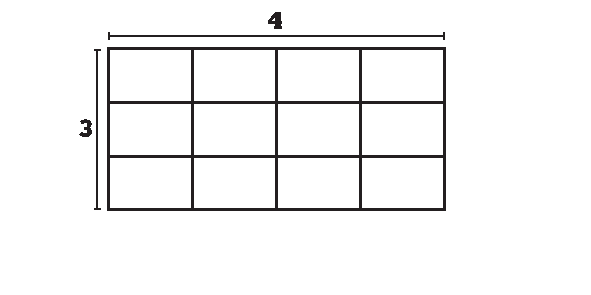
\includegraphics[scale=0.85]{pictures/Kuva2-4-3x4.pdf}
\end{center}
    
Kaikki luvut ovat jaollisia itsellään ja luvulla $1$. Esimerkiksi $7=7 \cdot 1=1 \cdot 7$, joten $7$ on jaollinen luvuilla $1$ ja $7$.
    
\laatikko{
	\termi{alkuluku}{Alkuluku} on ykköstä suurempi kokonaisluku, joka ei ole jaollinen muilla positiivisilla kokonaisluvuilla kuin luvulla $1$ ja itsellään.
}
    
    Esimerkiksi luvut 2, 3, 5, 7, 11, 13, 17 ja 19 ovat alkulukuja.
    kutsutaan alkutekijöiksi.
    
    \laatikko{
    \textbf{Aritmetiikan peruslause}
    
    Jokainen ykköstä suurempi kokonaisluku voidaan esittää yksikäsitteisesti alkulukujen tulona.
    }
    
   Aritmetiikan peruslause todistetaan kurssilla Logiikka ja lukuteoria.
    
    Esimerkiksi luku $84$ voidaan kirjoittaa muodossa $2\cdot 2\cdot 3\cdot 7$. Kokeilemalla havaitaan, että 2, 3, ja 7 ovat kaikki alkulukuja. Aritmetiikan peruslauseen nojalla tiedetään, että tämä on ainoa tapa kirjoittaa $84$ alkulukujen tulona -- mahdollista kerrottavien termien järjestyksen vaihtoa lukuunottamatta.
    
    %Kun luku $84$ esitetään muodossa $2\cdot 2\cdot 3\cdot 7$ on tapana sanoa, että se on \emph{jaettu alkutekijöihin}. Alkutekjät esitetään yleensä kasvavassa numerojärjestyksessä. Jos sama luku esiintyy tekijöissä useampaan kertaan, on se yleensä yleensä tapana merkitä potenssina. Tällöin luku $84$ voitaisiin kirjoittaa tekijöihin jaettuna $2^2\cdot 3\cdot 7$ ja luku $96$ muodossa $2\cdot 2\cdot 2\cdot 2\cdot 2\cdot 3=2^5\cdot 3$.
    
    %Luvun alkutekijät voi löytää etsimällä luvulle ensin jonkin esityksen kahden luvun tulona. Näiden kahden luvun ei tarvitse olla alkulukuja. Sen jälkeen sama toistetaan näille kahdelle luvulle ja edelleen aina uusille luvuille, kunnes tulossa on jäljellä vain alkulukuja.
    
    %\begin{esimerkki}
    %Luvun $96$ alkutekijät voi löytää vaikkapa seuraavanlaisella ketjulla: $96 = 2 \cdot 48 = 2 \cdot (2 \cdot 24) = 2 \cdot 2 \cdot (6 \cdot 4) = 2 \cdot 2 \cdot (2 \cdot 3) \cdot (2 \cdot 2)$. Nyt jäljellä on vain alkulukuja ja saatu tulo voidaan kirjoittaa lyhennettynä $96 = 2^5 \cdot 3$.
    %\end{esimerkki}

\begin{tehtavasivu}

\begin{tehtava}
	Mitkä seuraavista luvuista ovat jaollisia luvulla $4$?
	Jos luku $a$ on jaollinen luvulla $4$, kerro, millä kokonaisluvulla $b$ pätee $a = 4 \cdot b$. \\
	\begin{alakohdatrivi}
		\alakohta{$1$}
		\alakohta{$12$}
		\alakohta{$13$}
		\alakohta{$2$}
		\alakohta{$-20$}
		\alakohta{$0$}
	\end{alakohdatrivi}
	\begin{vastaus}
		\begin{alakohdat}
			\alakohta{Ei ole jaollinen luvulla $4$}
			\alakohta{On jaollinen luvulla $4$, $12 = 4 \cdot 3$}
			\alakohta{Ei ole jaollinen luvulla $4$}
			\alakohta{Ei ole jaollinen luvulla $4$}
			\alakohta{On jaollinen luvulla $4$, $-20 = 4 \cdot (-5)$}
			\alakohta{On jaollinen luvulla $4$, $0 = 4 \cdot 0$} 
		\end{alakohdat}
    \end{vastaus}
\end{tehtava}

\begin{tehtava}
    Jaa seuraavat luvut alkutekijöihin. \\
	\begin{alakohdatrivi}
		\alakohta{$12$}
		\alakohta{$15$}
		\alakohta{$28$}
		\alakohta{$30$}
		\alakohta{$64$}
		\alakohta{$90$}
		\alakohta{$100$}
	\end{alakohdatrivi}
    \begin{vastaus}
		\begin{alakohdat}
			\alakohta{$12 = 2^2 \cdot 3$}
			\alakohta{$15 = 3 \cdot 5$}
			\alakohta{$28 = 2^2 \cdot 7$}
			\alakohta{$30 = 2 \cdot 3 \cdot 5$}
			\alakohta{$64 = 2^6$}
			\alakohta{$90 = 2 \cdot 3^2 \cdot 5$}
			\alakohta{$100 = 2^2 \cdot 5^2$}
		\end{alakohdat}
    \end{vastaus}
\end{tehtava}

\end{tehtavasivu}
